\mysubsection{Sarah Häfele}{Möglichkeiten zur Weiterentwicklung}

Rhythmische Geschicklichkeitspiele sind heutzutage bei PC- wie auch bei Konsolen-Nutzern beliebt. Als Beispiel sollen hier Spiele wie \textit{Guitar Hero}, \textit{Audiosurf} oder das kürzlich erschienene \textit{Crypt of the Necrodancer} genannt werden. Da die Installation BlinkenTiles jedoch nur mit vollem Körpereinsatz funktioniert, können schnellere Challenges nur durch langes Üben geschafft werden. Es zeigte sich, dass schon allein der Freestyle Modus die Begeisterung der Besucher weckte. Um längerfristiger in einem öffentlichen Bereich stehen zu können, müsste es jedoch eine größere Auswahl an Liedtiteln geben und die Darstellung müsste verbessert werden (siehe \autoref{ssec:Praxis}. Die Installation lebt vor allem durch die Personen, die sich trauen auf so einer Matrix öffentlich zu agieren. In der medienaffinen Fakultät Digitale Medien ist dies kein großes Problem, wie der Tag der Medien bewies, in einem anderen Ort der Öffentlichkeit könnte dies jedoch anders aussehen. Besonders Kinder und Jugendliche sind hier dann anzusprechen. Mit den genannten Optimierungen und Anpassungen kann die Installation jedoch leicht in Einkaufszentren, in (Kunst-)Museen oder für Veranstaltungen verwendet werden. Das Potential liegt hier im gemeinsamen, kreativen Musizieren, ohne jegliche Vorkenntnisse vorzeigen zu müssen. Die Installation zu entwerfen und in Betrieb zu sehen hat uns noch etwas anderes gezeigt: die Vielfalt der Fakultät Digitale Medien.

\subsubsection{Impressionen Tag der Medien}
Zum Abschluss noch einige Fotos vom Aufbau und vom Tag der Medien. Im Anhang dazu finden sich die technischen Skizzen, die, teilweise veraltet, die Testaufbauten dokumentieren und der Projektgruppe als Planungshilfe dienten.

\begin{figure}[htbp]
	\centering
		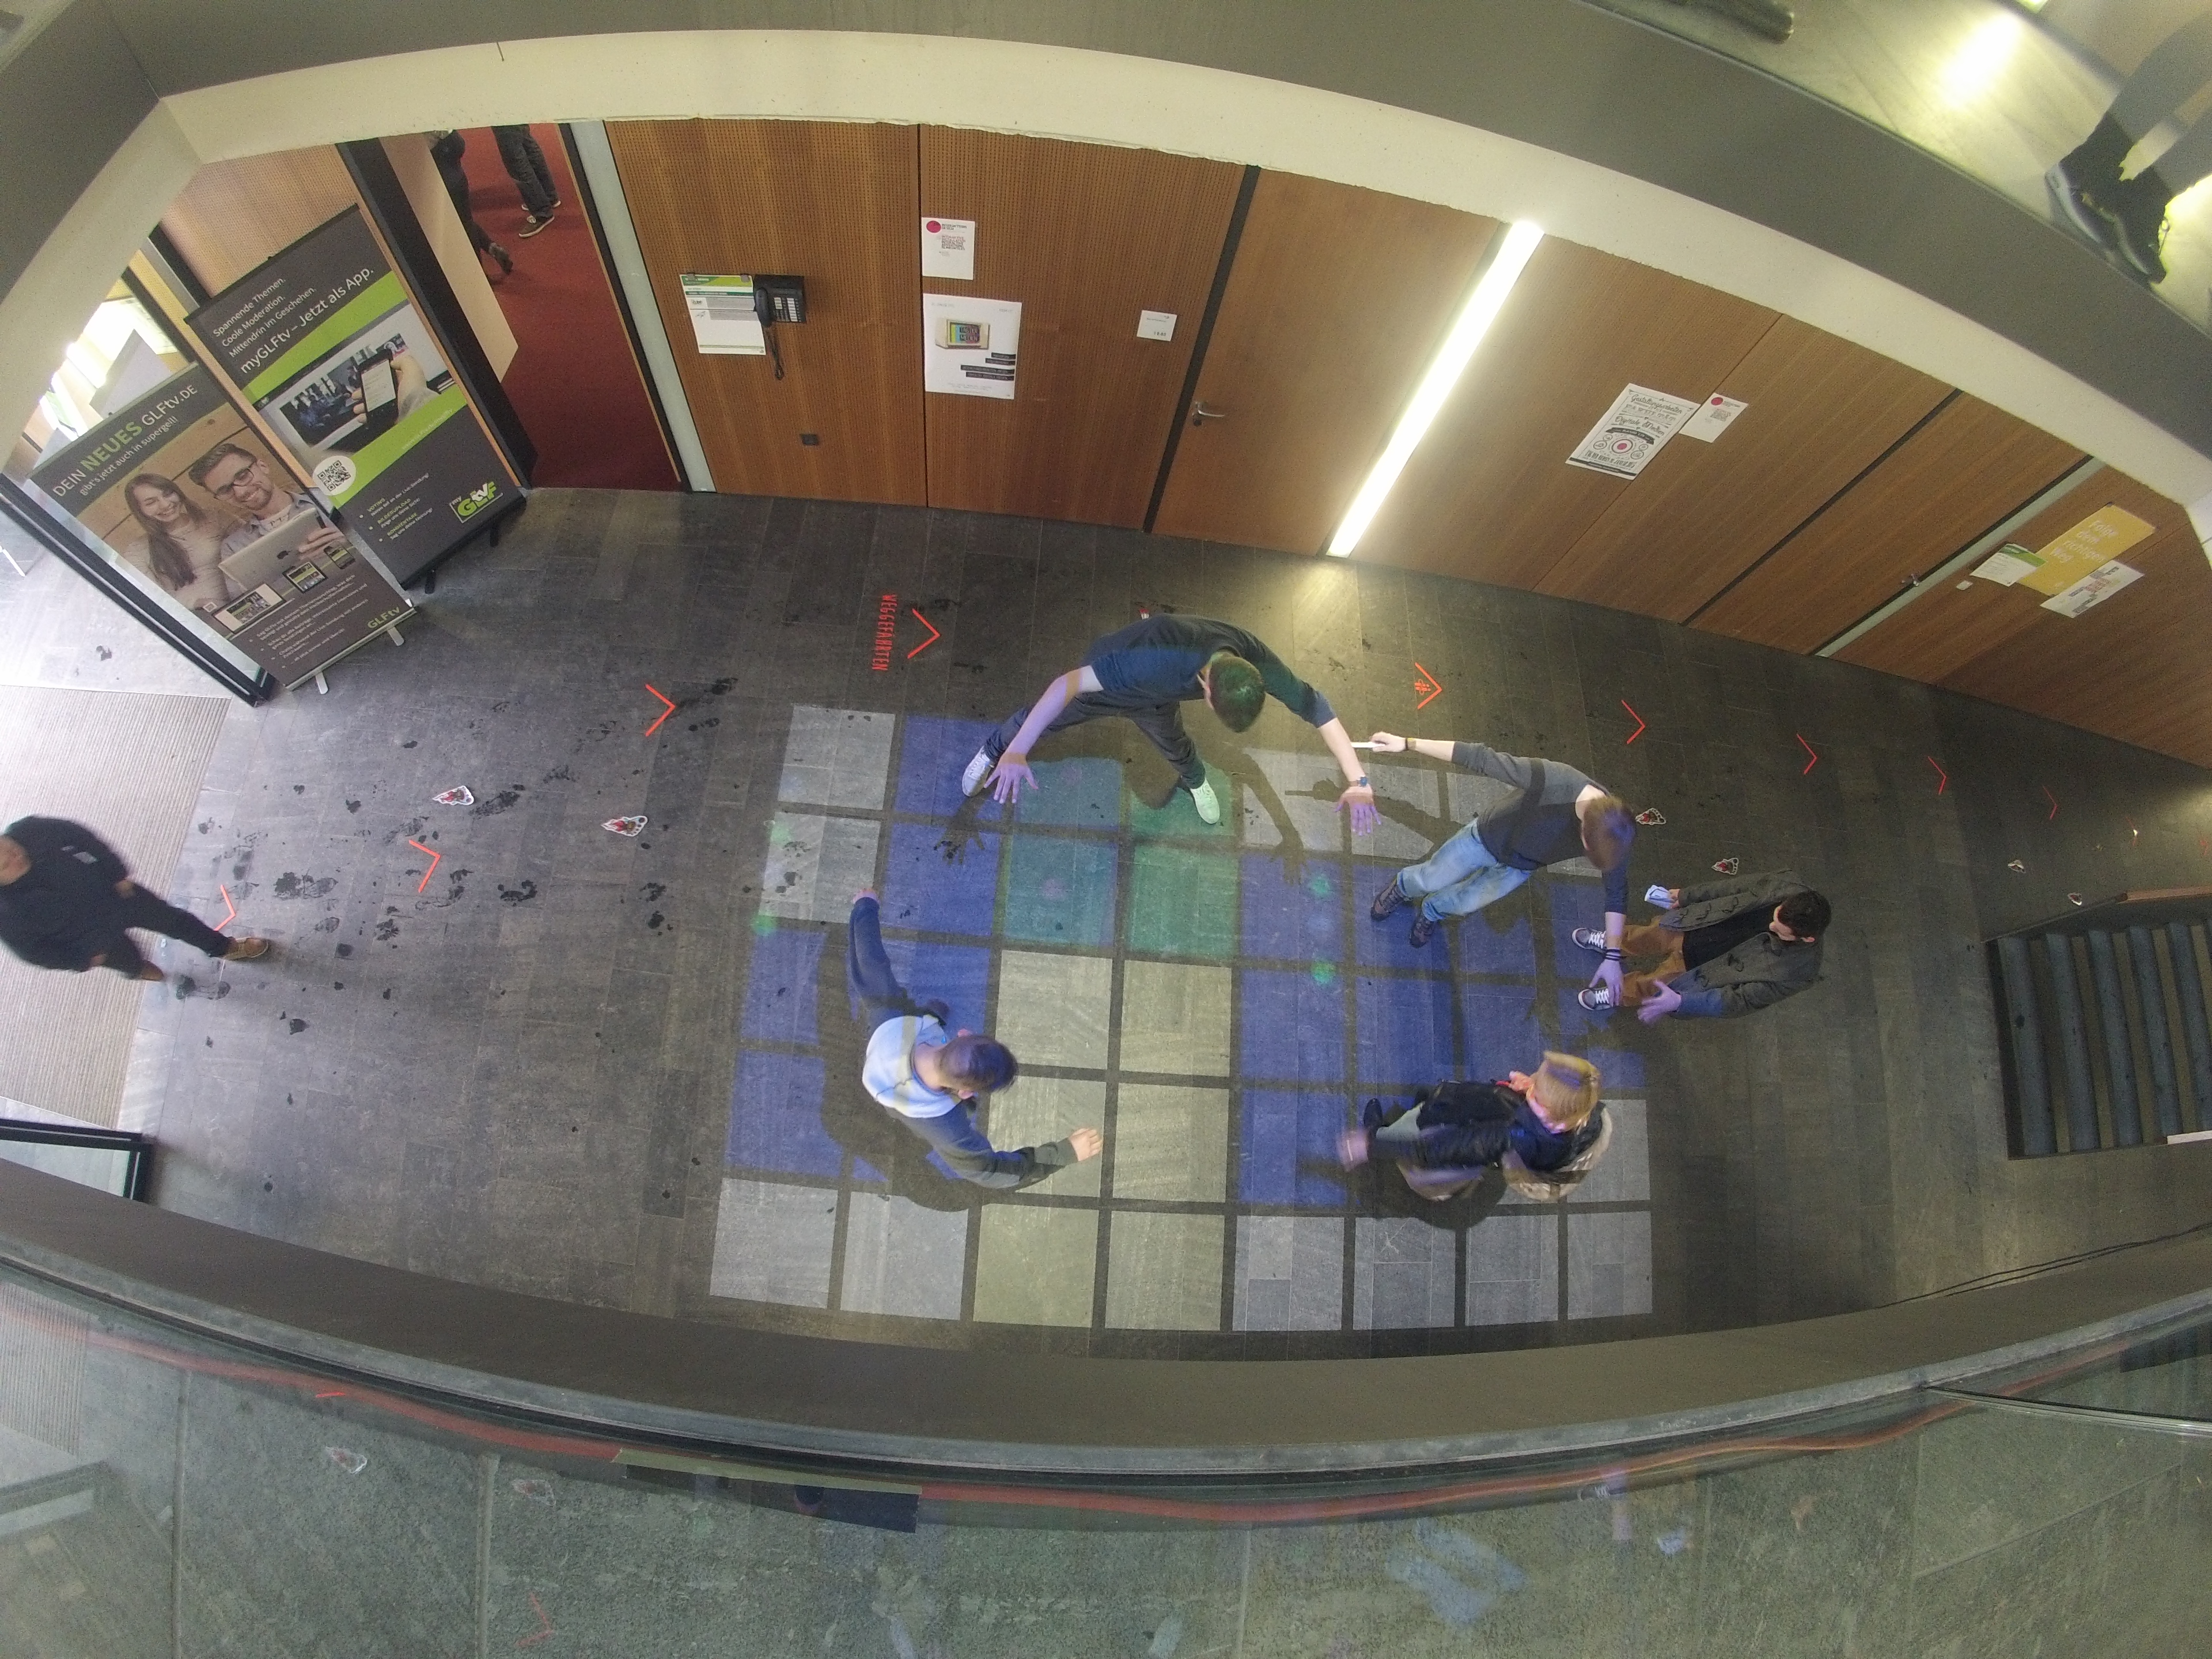
\includegraphics[width=0.9\textwidth]{images/TdM1.jpg}
	\caption{Installation von oben}
	\label{fig:TdM1}
\end{figure}

\begin{figure}[htbp]
	\centering
		\includegraphics[width=0.9\textwidth]{images/TdM2.jpg}
	\caption{Erdgeschoss (Foto: Ramazan Gündogdu)}
	\label{fig:TdM2}
\end{figure}

\subsubsection{Impressionen Erste Tests}